\begin{figure}[ht]
    \centering
    % Subfigure 1
    \begin{subfigure}{0.32\textwidth}
        \centering
        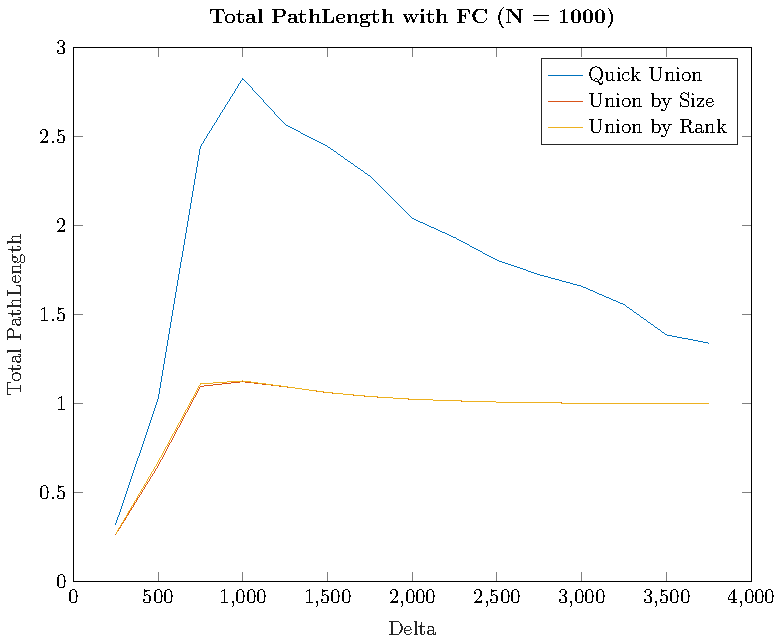
\includegraphics[width=\textwidth]{../images/plotFCFull1000_PathLength.pdf}
        \caption{Path Lengths with different union strategies with $n = 1000$}
    \end{subfigure}%
    \hfill
    % Subfigure 2
    \begin{subfigure}{0.32\textwidth}
        \centering
        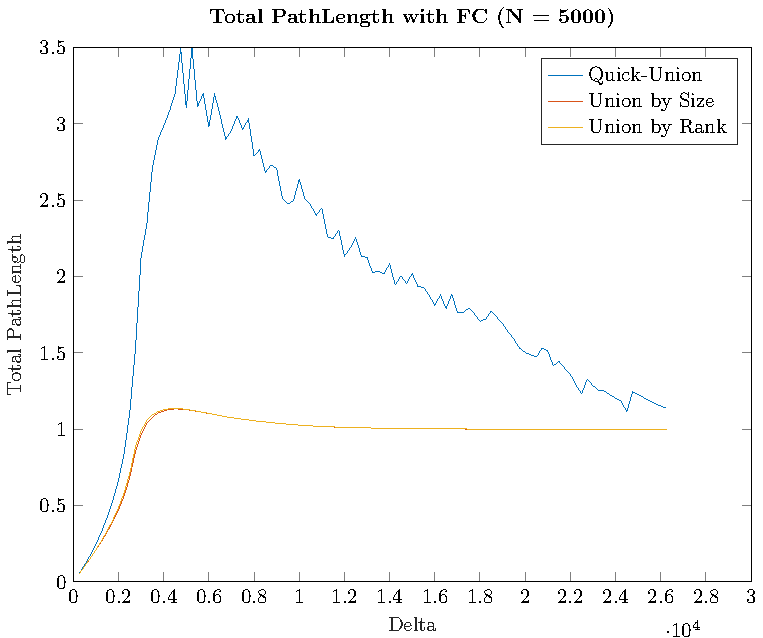
\includegraphics[width=\textwidth]{../images/plotFCFull5000_PathLength.pdf}
        \caption{Path Lengths with different union strategies with $n = 5000$}
    \end{subfigure}%
    \hfill
    % Subfigure 3
    \begin{subfigure}{0.32\textwidth}
        \centering
        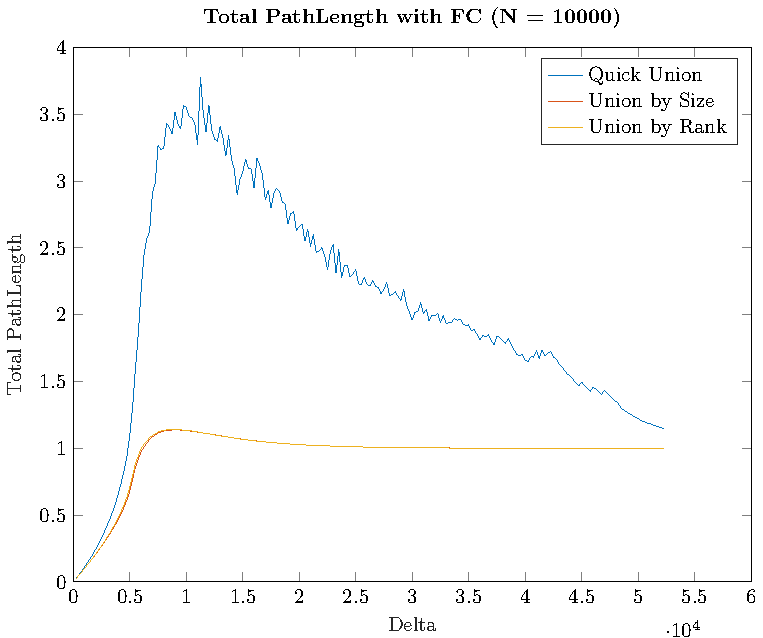
\includegraphics[width=\textwidth]{../images/plotFCFull10000_PathLength.pdf}
        \caption{Path Lengths with different union strategies with $n = 10000$}
    \end{subfigure}

    \caption{Total Path Length normalized with Full Compression}
    \label{fig:tplFC}
\end{figure}

\begin{figure}[ht]
    \centering
    % Subfigure 1
    \begin{subfigure}{0.32\textwidth}
        \centering
        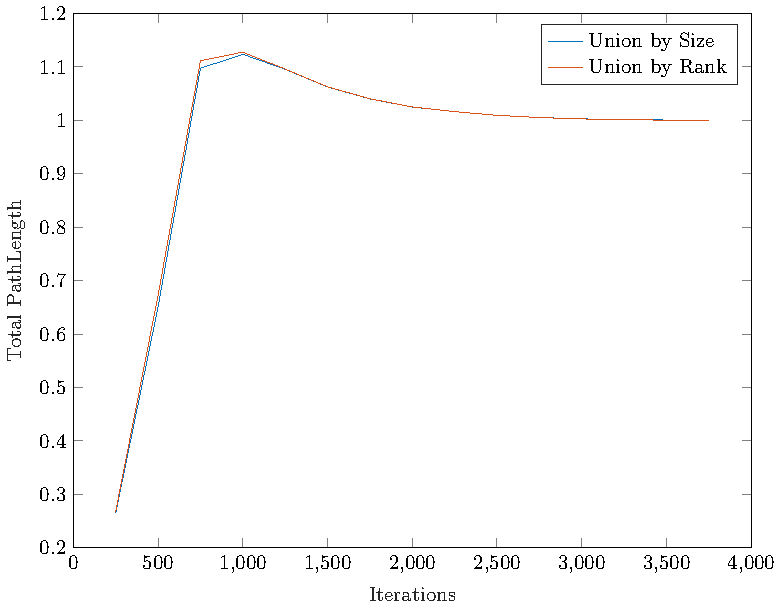
\includegraphics[width=\textwidth]{../images/plotFCNonFull1000_PathLength.pdf}
        \caption{Path Lengths with different union strategies with $n = 1000$}
    \end{subfigure}%
    \hfill
    % Subfigure 2
    \begin{subfigure}{0.32\textwidth}
        \centering
        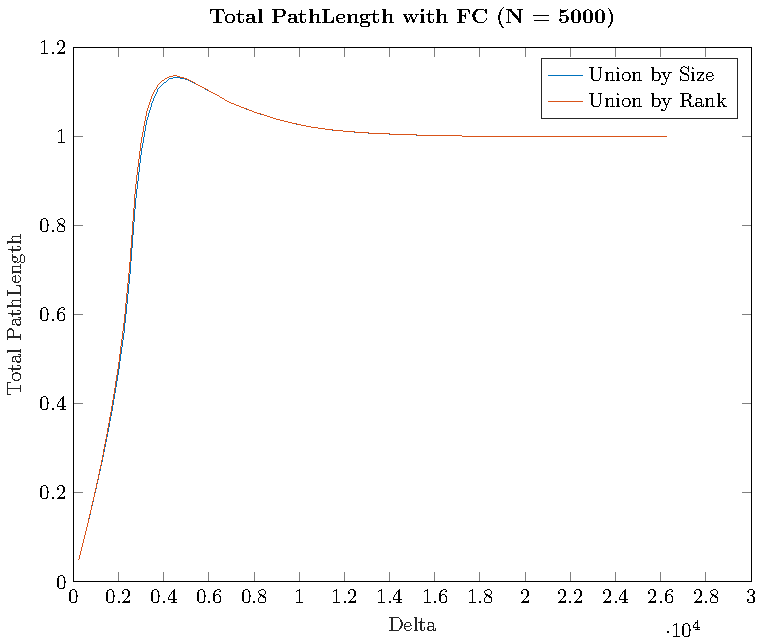
\includegraphics[width=\textwidth]{../images/plotFCNonFull5000_PathLength.pdf}
        \caption{Path Lengths with different union strategies with $n = 5000$}
    \end{subfigure}%
    \hfill
    % Subfigure 3
    \begin{subfigure}{0.32\textwidth}
        \centering
        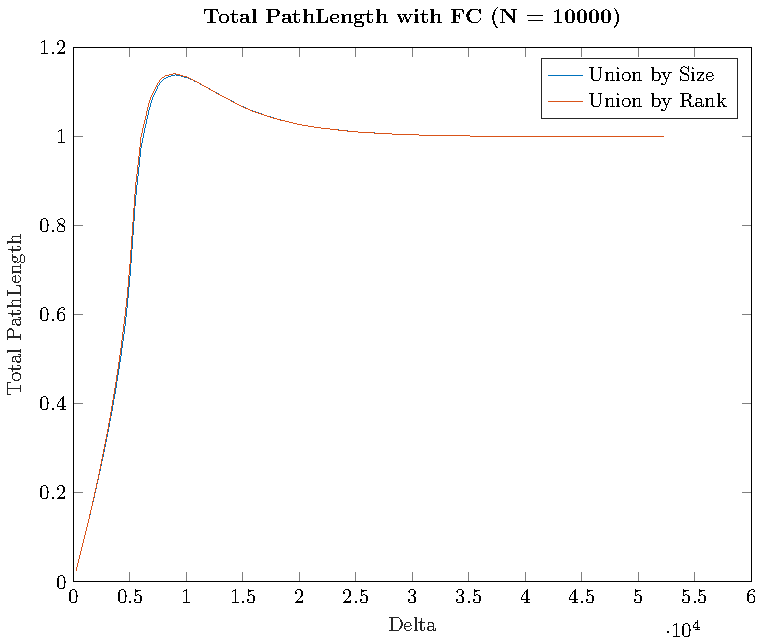
\includegraphics[width=\textwidth]{../images/plotFCNonFull10000_PathLength.pdf}
        \caption{Path Lengths with different union strategies with $n = 10000$}
    \end{subfigure}

    \caption{Total Path Length normalized with Full Compression without Quick-Union}
    \label{fig:tplFCNoQU}
\end{figure}

\begin{figure}[ht]
    \centering
    % Subfigure 1
    \begin{subfigure}{0.32\textwidth}
        \centering
        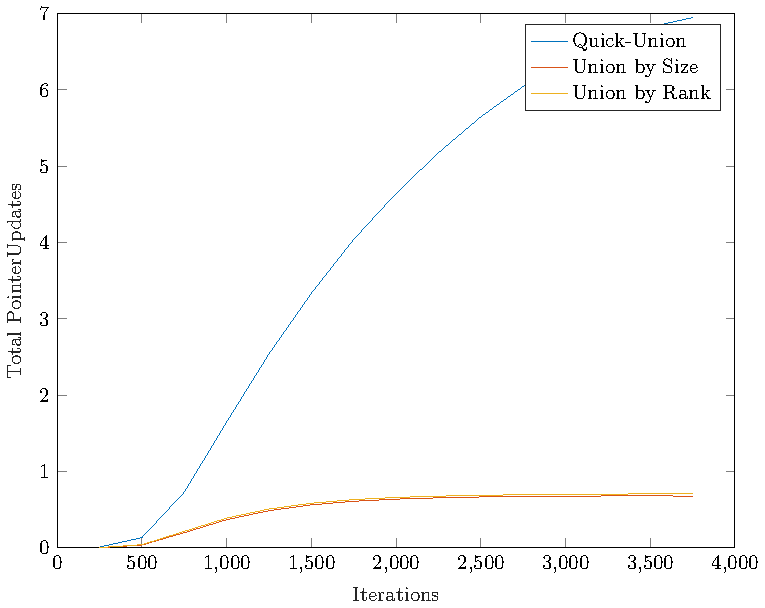
\includegraphics[width=\textwidth]{../images/plotFCFull1000_PointerUpdates.pdf}
        \caption{Pointer Updates with different union strategies with $n = 1000$}
    \end{subfigure}%
    \hfill
    % Subfigure 2
    \begin{subfigure}{0.32\textwidth}
        \centering
        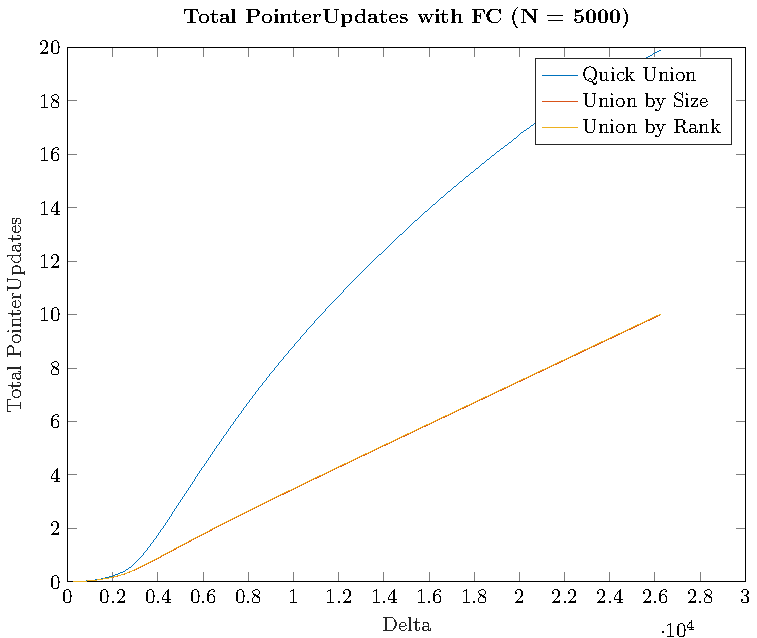
\includegraphics[width=\textwidth]{../images/plotFCFull5000_PointerUpdates.pdf}
        \caption{Pointer Updates with different union strategies with $n = 5000$}
    \end{subfigure}%
    \hfill
    % Subfigure 3
    \begin{subfigure}{0.32\textwidth}
        \centering
        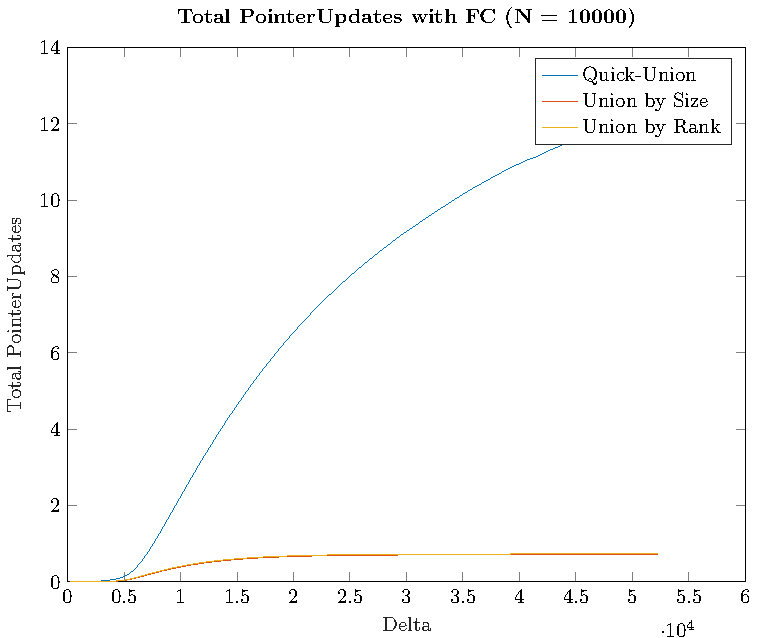
\includegraphics[width=\textwidth]{../images/plotFCFull10000_PointerUpdates.pdf}
        \caption{Pointer Updates with different union strategies with $n = 10000$}
    \end{subfigure}

    \caption{Total Pointer Update normalized with Full Compression}
    \label{fig:tpuFC}
\end{figure}


\begin{figure}[ht]
    \centering
    % Subfigure 1
    \begin{subfigure}{0.32\textwidth}
        \centering
        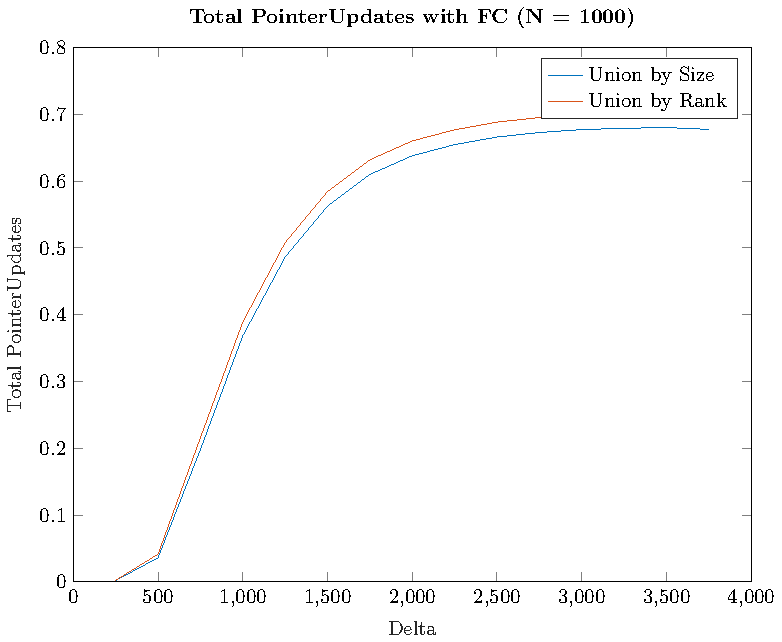
\includegraphics[width=\textwidth]{../images/plotFCNonFull1000_PointerUpdates.pdf}
        \caption{Pointer Updates with different union strategies with $n = 1000$}
    \end{subfigure}%
    \hfill
    % Subfigure 2
    \begin{subfigure}{0.32\textwidth}
        \centering
        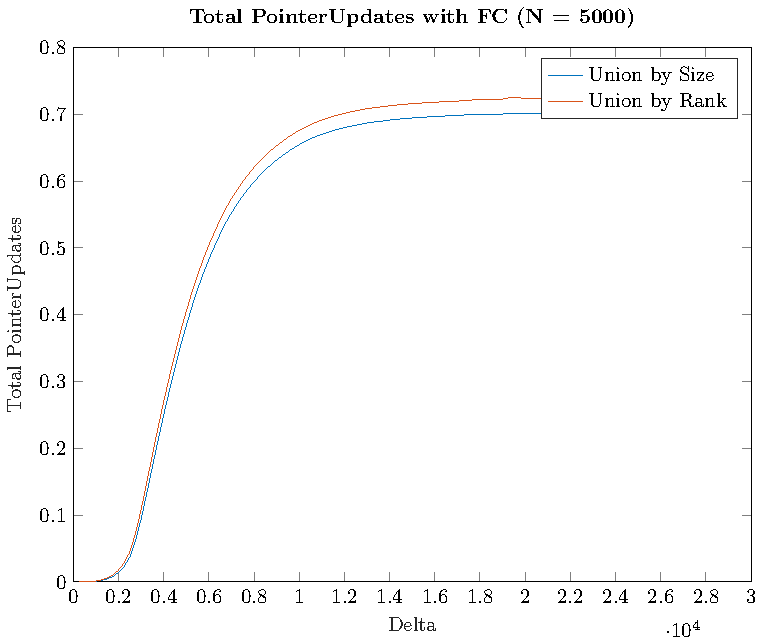
\includegraphics[width=\textwidth]{../images/plotFCNonFull5000_PointerUpdates.pdf}
        \caption{Pointer Updates with different union strategies with $n = 5000$}
    \end{subfigure}%
    \hfill
    % Subfigure 3
    \begin{subfigure}{0.32\textwidth}
        \centering
        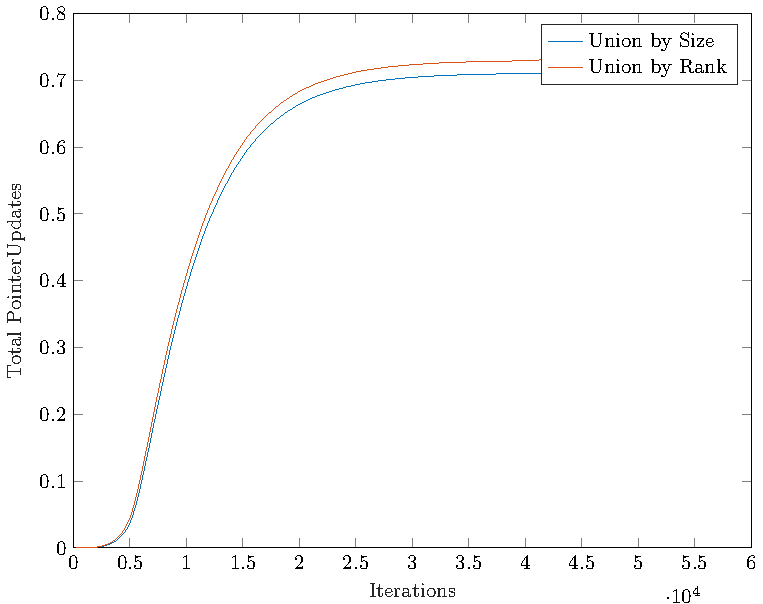
\includegraphics[width=\textwidth]{../images/plotFCNonFull10000_PointerUpdates.pdf}
        \caption{Pointer Updates with different union strategies with $n = 10000$}
    \end{subfigure}

    \caption{Total Pointer Update normalized with Full Compression without Quick-Union}
    \label{fig:tpuFCNoQU}
\end{figure}
